%************************************************
%************************************************
\section{Introduction}
\label{sec:introduction}
%************************************************
%************************************************

\begin{figure}[tb]
  \centering
  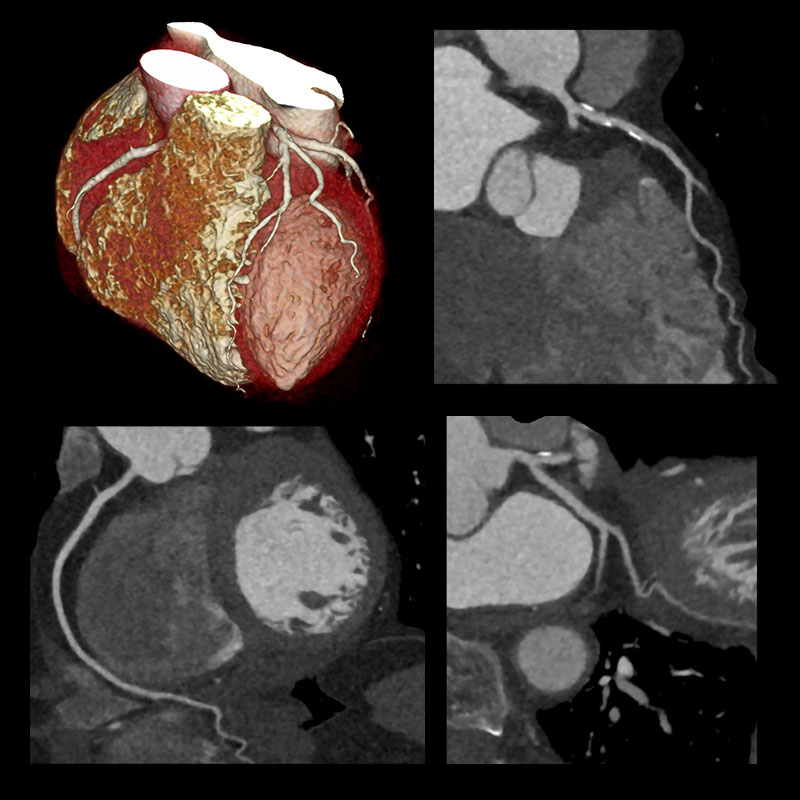
\includegraphics[width=0.7\linewidth]{gfx/my_images/intro_ct.jpg}
  \caption[Four panel view of cardiac CT]{
    Four panel view of cardiac CT imaging. Panels show: 3D rendering of the heart 
    (top left), axial (bottom left), sagital (top right) and coronal (bottom right)
    views. 
  Image source: LaBarbera and Donnino \cite{labarberra2008_NoninvasiveCardiacImaging}}
  \label{fig:intro_ct}
\end{figure}





\paragraph{This section show the use of acronyms package}
Cardiovascular diseases (\acs{CVD}) have been identified as the leading cause
of death in the developed world
\cite{nichols2012_Europeancardiovasculardisease,worldhealthorganization2017_top10causes}.
Diagnosis and treatment of \acp{CVD} has significantly improved in recent years
due to the advances in cardiovascular imaging technologies. However, fast and
accurate extraction of clinically relevant data from cardiovascular images
still presents a challenge. Clinically relevant data is necessary for both the
diagnosis of \acp{CVD} and for the planning of medical procedures. The field
where researchers develop methods and algorithms for extraction of such data
from medical images is called medical image analysis.  This report is focused
on the state-of-the-art methods for the segmentation and analysis of the left
atrium and the left atrial appendage.  The methods presented in this report are
aimed to aid physicians in planning and execution of a procedure that reduces
the risk of stroke -- the \acf{LAA} occlusion. 



%************************************************
%************************************************
\section{Figures and subfigures}
\label{sec:bg_anatomy_laa}
%************************************************
%************************************************
Figure \ref{fig:intro_ct} shows a figure without subfigures.
Figure \ref{fig:bg_laa_outside} shows a figure with subfigures without labels
for subfigures. Figure \ref{fig:bg_laa_morphologies} shows a figure with
subfigures with labels for every subfigure. Cactus type is shown in Figure
\ref{fig:bg_laa_morphologies_cactus}, while a different type called windsock is 
shown in Figure \ref{fig:bg_laa_morphologies_windsock}.

\begin{figure}[t]
  \myfloatalign
  \subfloat[] {
    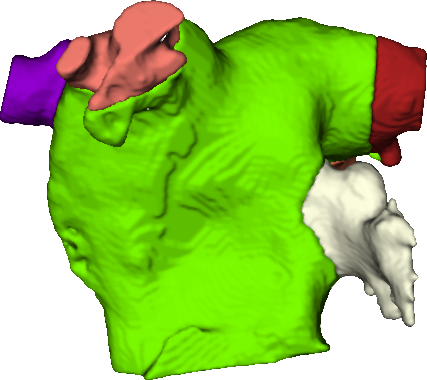
\includegraphics[width=.37\linewidth]{gfx/my_images/laa1_siemens.png}
  } \quad
  \subfloat[] {
    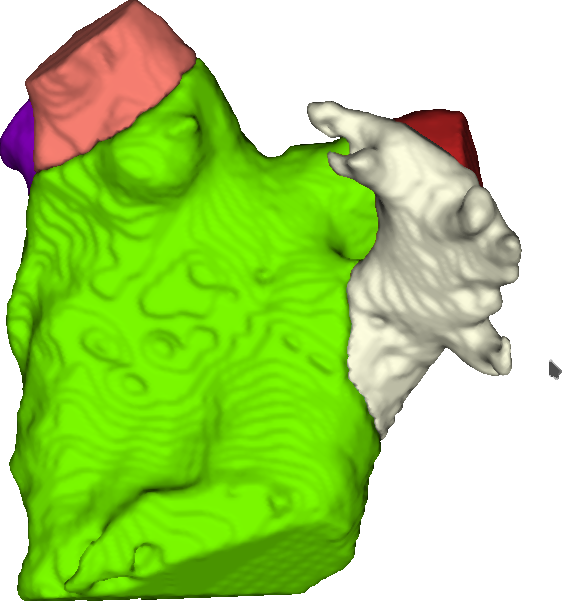
\includegraphics[width=.37\linewidth]{gfx/my_images/laa2_siemens.png}
  } \\
  \subfloat[] {
    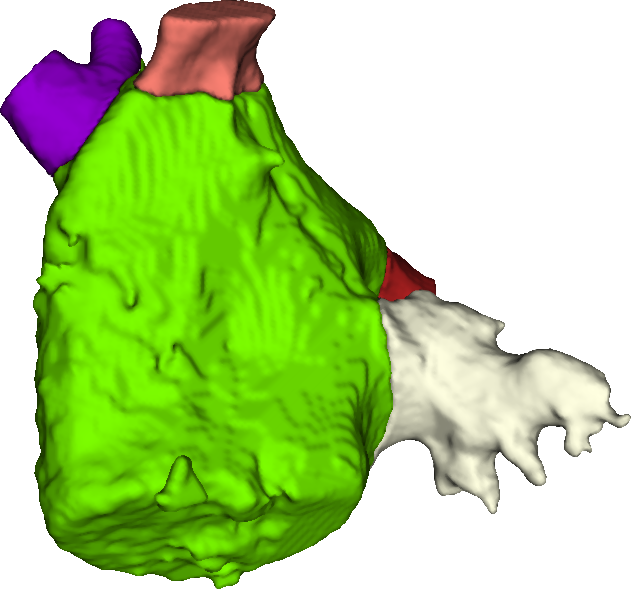
\includegraphics[width=.37\linewidth]{gfx/my_images/laa3_siemens.png}
  } \quad
  \subfloat[] {
    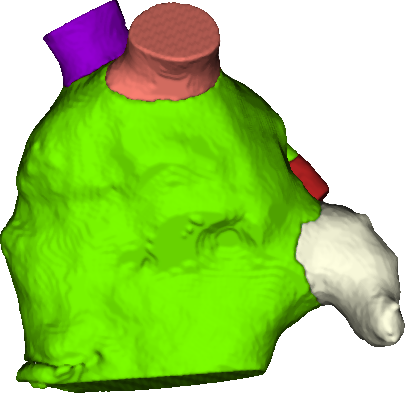
\includegraphics[width=.37\linewidth]{gfx/my_images/laa4_siemens.png}
  }
  \caption[LAA examples]{Renderings of \acp{LAA} (white) in posterior view with the 
    left atrium (green) and pulmonary veins visible.  Segmentation results from the 
    LASC datasets \cite{tobon-gomez2015_BenchmarkAlgorithmsSegmenting}
  }
  \label{fig:bg_laa_outside}
\end{figure}



\begin{table}[t]
  \centering
  \caption{Criteria for defining the \laa lobes. Reprinted from Veinot et al. \cite{veinot1997_AnatomyNormalLeft}.}
  \label{tab:bg_laa_lobes_criteria}
  \begin{tabular}{IL}
    \hline\noalign{\smallskip}
    \multicolumn{2}{l}{Criteria for an \laa lobe according to \cite{veinot1997_AnatomyNormalLeft} }\\
    \noalign{\smallskip}\hline\noalign{\smallskip}
    (1) & {\footnotesize it was a visible outpouching from the main tubular body of the LAA, usually
    demarcated by an external crease; } \\
    (2) & {\footnotesize  it was internally capable of admitting a
    2-mm probe (ie, it was not simply a tag of external adipose tissue); } \\
    (3) & {\footnotesize it was
    occasionally but not necessarily associated with a change in direction of the
    main tubular body of the LAA; } \\
    (4) & {\footnotesize it could lie in a different anatomic plane
    than the main tubular body; and } \\
    (5) & {\footnotesize by definition, the LAA must have at least
    one lobe (ie, a tubular body with a blind-ending sac).} \\
    \noalign{\smallskip}\hline\noalign{\smallskip}
  \end{tabular}
\end{table}



\begin{figure}[t]
  \myfloatalign
  \subfloat[Cactus] {
    \label{fig:bg_laa_morphologies_cactus}  
    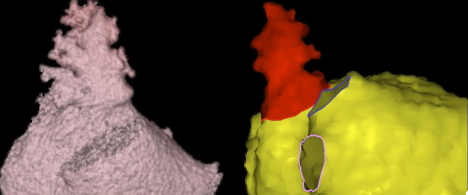
\includegraphics[width=.48\linewidth]{gfx/my_images/laa_cactus.png}
  } 
  \subfloat[Chicken wing] {
    \label{fig:bg_laa_morphologies_chicken}  
    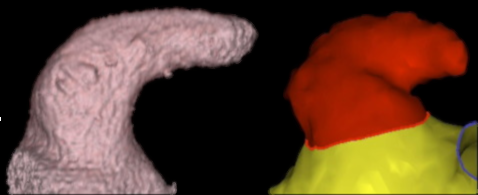
\includegraphics[width=.48\linewidth]{gfx/my_images/laa_chickenwing.png}
  } \\
  \subfloat[Windsock] {
    \label{fig:bg_laa_morphologies_windsock}  
    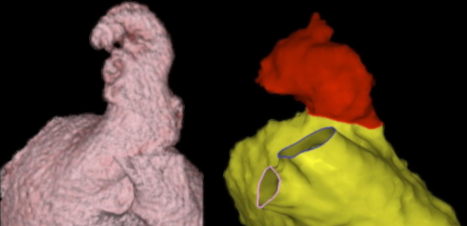
\includegraphics[width=.48\linewidth]{gfx/my_images/laa_windsock.png}
  } 
  \subfloat[Cauliflower] {
    \label{fig:bg_laa_morphologies_cauliflower}  
    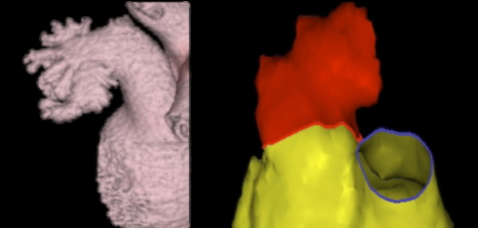
\includegraphics[width=.48\linewidth]{gfx/my_images/laa_cauliflower.png}
  }
  \caption[LAA morphology types]{Types of \laa morphology. Each subfigure shows 
    the rendering of a CT dataset (left) and an MRI dataset (right).
    Image source: Di Biase et al. \cite{dibiase2012_DoesLeftAtrial}.
  }
  \label{fig:bg_laa_morphologies}  
\end{figure}









\begin{table}[t]
  \centering
  \caption{Criteria for each morphology type. Table from Wang et al. \cite{wang2010_LeftAtrialAppendage}.}
  \label{tab:bg_laa_morphology}
  \begin{tabular}{IL}
    \hline\noalign{\smallskip}
    \multicolumn{2}{l}{ LAA with obvious bend  }\\
    \noalign{\smallskip}\hline\noalign{\smallskip}
    1 & \emph{The ChickenWing LAA} {\footnotesize is an anatomy whose main characteristic is an obvious bend in the proximal or middle part of the dominate lobe or folding back of the LAA anatomy on itself at some distance from the perceived LAA ostium. This LAA type may vary with or without secondary lobes or twigs, with the different measured distance to this bend as well as with the different orientation (anterior, superior, inferior, etc.) of the bend relative to the main lobe.} \\
    \noalign{\smallskip}\hline\noalign{\smallskip}
    \multicolumn{2}{l}{ LAA without obvious bend  }\\
    \noalign{\smallskip}\hline\noalign{\smallskip}
    2 & \emph{The WindSock LAA}  {\footnotesize  is an anatomy in which 1 dominant lobe of sufficient length is the primary structure. Variations of this LAA type arise with the location and number of secondary or even tertiary lobes arising from the dominate lobe in inferior direction.} \\
    3 & \emph{The Cauliflower LAA} {\footnotesize  is an anatomy whose main characteristic is an LAA that has limited overall length with more complex internal characteristics. Variations of this LAA type are demonstrated by a more irregular shape of the perceived LAA ostium (oval vs. round), the number of significant lobes present and lack of 1 dominate lobe and the close proximity of internal separations or prominent pectinate ridges to the perceived LAA ostium.} \\
    4 & \emph{The Cactus LAA} {\footnotesize  is an anatomy whose main characteristic is a dominant central lobe with secondary lobes extending from the central lobe in both superior and inferior directions. Variations of this type relate to the number, location and orientation of the secondary lobes. This type of LAA may present like a fork with a dominant lobe and with 2 or 3 secondary lobes at the top of LAA. } \\
    \noalign{\smallskip}\hline\noalign{\smallskip}
  \end{tabular}
\end{table}


\subsection{Afterpage package}%
\label{sec:afterpage_package}
Afterpage package enables you to force the figure to go to the next page. Only
thing you have to do is wrap the figure in the  
environment.
